\documentclass[times, utf8, diplomski, numeric]{fer}

\usepackage{booktabs}
\usepackage{listings}

\usepackage{xcolor}
\usepackage{color, colortbl}
\usepackage{pgfplotstable}
\usepackage{pgfplots}

\usepackage{url}
\def\UrlBreaks{\do/\do-}
\usepackage{breakurl}
\usepackage[breaklinks]{hyperref}

\hypersetup{
	colorlinks,
	linkcolor={black},
	citecolor={black},
	urlcolor={black}
}

\definecolor{codegray}{rgb}{0.5,0.5,0.5}
\definecolor{codegreen}{rgb}{0,0.6,0}
\definecolor{codepurple}{rgb}{0.58,0,0.82}
\definecolor{lightblue}{rgb}{0.7,0.99,0.99}

\lstdefinestyle{mystyle}{
	frame=single,   
	commentstyle=\color{codegreen},
	keywordstyle=\color{magenta},
	stringstyle=\color{codepurple},
	basicstyle=\ttfamily,
	breakatwhitespace=false,         
	breaklines=true,                 
	captionpos=b,                    
	keepspaces=true,                 
	showspaces=false,                
	showstringspaces=false,
	showtabs=false,                  
	tabsize=2
}

\lstset{style=mystyle}

\renewcommand*{\lstlistingname}{Isječak koda}
\renewcommand*\lstlistlistingname{Popis isječaka koda}

\begin{document}

% TODO: Navedite broj rada.
%\thesisnumber{358}

% TODO: Navedite naslov rada.
%\title{Sustav za udaljeni nadzor u poljoprivredi temeljen na platformi ESP32-C3 i AWS-uslugama}

% TODO: Navedite vaše ime i prezime.
%\author{Jelena Gavran}

%\maketitle

% Ispis stranice s napomenom o umetanju izvornika rada. Uklonite naredbu \izvornik ako želite izbaciti tu stranicu.
%\izvornik

% Dodavanje zahvale ili prazne stranice. Ako ne želite dodati zahvalu, naredbu ostavite radi prazne stranice.
\zahvala{}

\tableofcontents

\begingroup
\renewcommand*\listfigurename{Popis slika}
\listoffigures
\addcontentsline{toc}{chapter}{\lstlistlistingname}
\lstlistoflistings
\listoftables
\endgroup

\chapter{Uvod}

Internet stvari \engl{Internet of Things - IoT} brzo je rastuća tehnologija koja urbani svijet pretvara u potpuno mrežno povezani sustav visoke tehnologije. Uz sve veću popularnost, potražnju i rastuće zahtjeve na IoT tehnologiju, sustavi generiraju sve veću količinu podataka koju je gotovo nemoguće obraditi lokalno. Tom je izazovu doskočila tehnologija računarstva u oblaku \engl{cloud computing} koja pruža softver, alate i infrastrukturu preko interneta umjesto lokalnog upravljanja. Računanje u oblaku može pružiti skalabilnost i dostupnost potrebnu za obradu i pohranu velike količine podataka koju stvaraju IoT sustavi. Osim toga, računanje u oblaku može pomoći smanjiti troškove upravljanja IoT sustavima. 

U posljednjih nekoliko godina, poljoprivreda je doživjela značajne promjene zahvaljujući integraciji naprednih tehnologija poput interneta stvari i računarstva u oblaku. Ove tehnologije omogućuju razvoj moderne poljoprivrede koja koristi različite senzore i podatke radi optimizacije proizvodnih procesa i povećanja efikasnosti. IoT u poljoprivredi omogućuje povezivanje fizičkih uređaja i senzora s internetom, čime se prikupljaju podaci o stanju na poljoprivrednim gospodarstvima, stanju usjeva i učinkovitosti rada. Računarstvo u oblaku pruža infrastrukturu za obradu i analizu tih podataka u stvarnom vremenu, što omogućuje poljoprivrednicima da donose informirane odluke i poboljšavaju svoj tijek rada. 

Za razvoj poljoprivrednih IoT sustava potrebni su ugradbeni računalni sustavi s mogućnošću bežičnog povezivanja, primarno Wi-Fi komunikacije. Serija mikrokontrolera ESP32 tvrtke \textit{Espressif} jedan je od danas najpopularnijih izbora među bežičnim uređajima zbog niske potrošnje, visoke otpornosti na temperature te najvažnije, jednostavnom bežičnom povezivosti \cite{top_iot_boards}. Jedan takav integrirani sklop jest ESP32-C3 koji pruža Bluetooth i Wi-Fi povezivanje. Sklop je integriran u nekoliko modula, koji su pak dio razvojnih sustava koje proizvodi tvrtka \textit{Espressif}. Za izradu ovog rada odabran je razvojni sustav ESP32-C3-DevKitM-1. Isto tako, usluga računarstva u oblaku mora biti jednostavna, intuitivna, pouzdana te najvažnije, skalabilna. Platforma AWS tvrtke \textit{Amazon} ističe se kao jedan od najkorištenijih sustava za računarstvo u oblaku. Također nudi brojne mogućnosti za umrežavanje IoT sustava. Isto tako, potrebna je i prikladna web aplikacija koja će pružiti kvalitetne vizualizacije prikupljenih podataka. Jedna takva interaktivna aplikacija jest Grafana, koja nudi široku paletu grafikona i sučelja za prikaz podataka. 

Rad je podijeljen u cjeline kako slijedi. U drugom poglavlju \textit{„Opis sustava i tehničkih zahtjeva“} objašnjen je koncept precizne poljoprivrede kao domene izrađenog sustava te je prikazana sklopovska i programska arhitektura rješenja, kao i zahtjevi koje je trebalo ispuniti. Treće poglavlje \textit{„Razvojni sustav ESP32-C3-DevKitM-1“} opisuje osnovne značajke korištenog razvojnog sustava kao ciljane hardverske platforme, a zatim su opisana svojstva Wi-Fi mreže te njene značajke koje podržava razvojni sustav. U četvrtom poglavlju \textit{„Amazon Web Services“} opisana je korištena platforma za računarstvo u oblaku i navedene su usluge koje nudi za razvoj IoT sustava. U petom poglavlju \textit{„Povezivanje razvojnog sustava i oblaka“} opisana je programska potpora za mikrokontroler i periferne uređaje te dio programske potpore za računarstvo u oblaku koja služi za povezivanje i komunikaciju s ugradbenim sustavom. Također je opisana infrastruktura potrebna za pohranu podataka na platformi. U šestom poglavlju \textit{„Web aplikacija“} opisana je infrastruktura razvijene web aplikacije na temelju platforme Grafana. Opisan je i alarmni sustav integriran u web aplikaciju.

\eject
%\chapter{Opis sustava i tehničkih zahtjeva}

\section{Opis problematike u poljoprivredi - WIP naslov potpoglavlja}

Moj problematični poljoprivredni sustav. Ovdje opisati sa čim se poljopvrivrednici bore, šta im smeta, potkrijepiti to tako linkovima, onda naći rješenja koja su im pomogla i kako im IoT poljoprivreda boosta productivity i poboljšava usjeve i tako to. 

\section{Zahtjevi na sustav i opis predloženog rješenja}

Ovdje je prikazana moja blok shema sustava koju trebam podrobnije opisati. 

\begin{figure}[ht]
	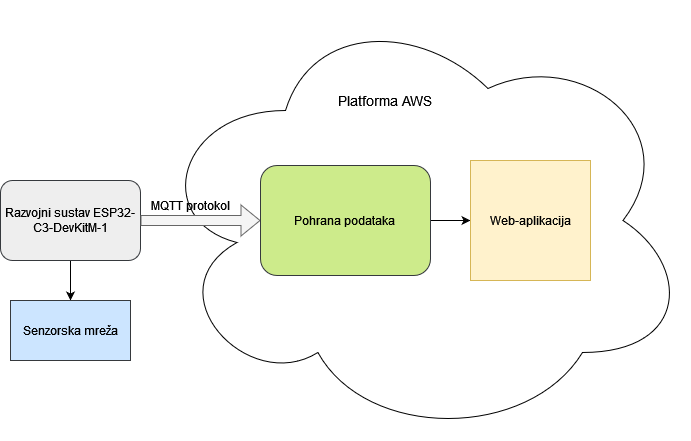
\includegraphics[width=\linewidth]{imgs/shema}
	\caption{Blok shema sustava}
	\label{fig:shema}
\end{figure}


\chapter{Zaključak}

Moj zaključak.

\eject

\bibliography{literatura}{}
\bibliographystyle{fer}

\title{Sustav za udaljeni nadzor u poljoprivredi temeljen na platformi ESP32-C3 i AWS-uslugama}
\begin{sazetak}
Ovo je moj hrvatski sažetak.

\kljucnerijeci{prva, druga, treća, ključna, riječ}
\end{sazetak}

% TODO: Navedite naslov na engleskom jeziku.
\engtitle{System For Remote Monitoring In Agriculture Based On ESP32-C3 Platform and AWS Services}
\begin{abstract}
This is my english abstract.

\keywords{first, second, third, key, word}
\end{abstract}

\end{document}
